\part{GTK}
\chapter{Ejemplo de una arquitectura de código de aplicación GTK}
\label{gtk-app-arch}

\emph{Este capítulo no está completamente terminado, puede ser difícil de entender sin ningún conocimiento sobre GTK u otro conjunto de herramientas de widgets. Y el capítulo no está bien integrado con los otros capítulos, la introducción y los capítulos de lectura adicional no se han adaptado, por ejemplo. Este capítulo se distribuye con la esperanza de que sea útil, pero SIN NINGUNA GARANTÍA; incluso sin la garantía implícita de COMERCIABILIDAD o APTITUD PARA UN PROPÓSITO EN PARTICULAR.}

%FIXME: vuelve a explicar qué es un "widget" y un "contenedor". Y agregue un glosario al final.

Para cualquier proyecto de programación, es importante diseñar correctamente la arquitectura de código general. Con Programación Orientada a Objetos, significa definir las clases principales. Este capítulo explica un buen ejemplo de una arquitectura de código para una aplicación GTK, observando una vista simplificada del editor de texto gedit \footnote{\url{https://wiki.gnome.org/Apps/Gedit}}.

gedit tiene una interfaz de documento con pestañas: se pueden abrir varios archivos en la misma ventana de gedit, en diferentes pestañas. Como veremos, esto se refleja en la arquitectura del código.

La Figura~\ref{fig:gedit-architecture} p.~\pageref{fig:gedit-architecture} muestra el esquema de la clase. Cada clase gedit en el esquema es una subclase de una clase GTK o GtkSourceView. (GtkSourceView \footnote{\url{https://wiki.gnome.org/Projects/GtkSourceView}} es una biblioteca que extiende el widget \lstinline{GtkTextView}; \lstinline{GtkTextView} es parte de GTK).

Repasaremos el esquema de la clase, explicando las clases paso a paso, comenzando por la parte superior. Esto permitirá presentar algunas de las clases GTK más importantes, no describiéndolas en detalle con muchos ejemplos de código, sino dando una descripción general de alto nivel.

\begin{figure}
  \begin{center}
    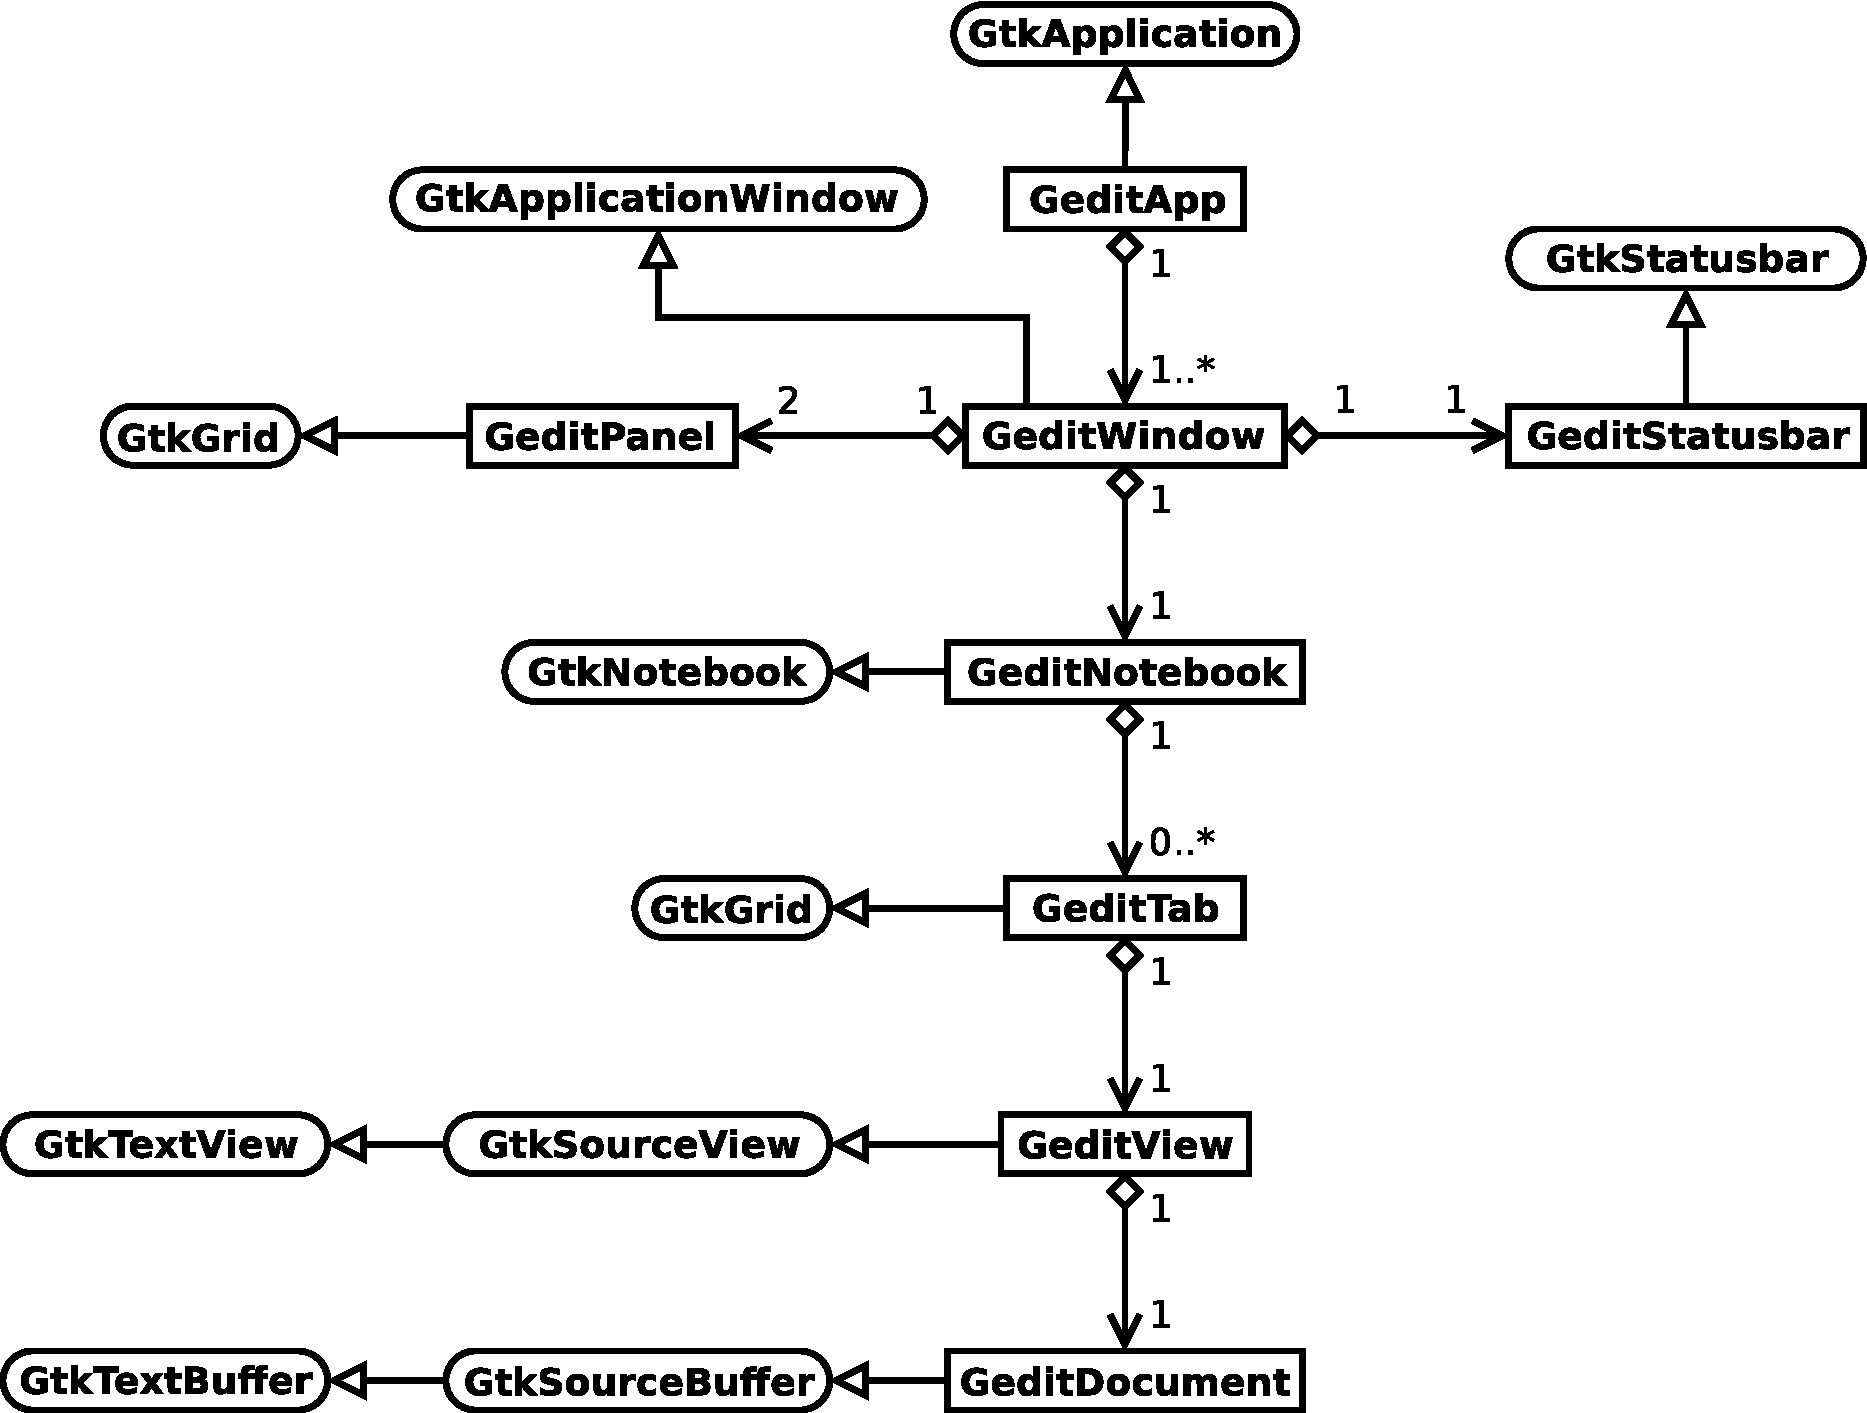
\includegraphics[width=\textwidth]{assets/img/gedit-architecture.pdf}
    \caption{Arquitectura de código simplificada del editor de texto gedit}
    \label{fig:gedit-architecture}
  \end{center}
\end{figure}

\section{La función main() y GeditApp}

Aunque no está representado en el esquema, el punto de entrada de una aplicación GTK --~como para todos los programas en C~-- es la función \lstinline{main()}. Para crear una aplicación GTK, lo principal que se debe hacer en \lstinline{main()} es crear una instancia de \lstinline{GtkApplication}, o una subclase de la misma. En el esquema vemos que \lstinline{GeditApp} es una subclase de \lstinline{GtkApplication}, por lo que la función \lstinline{main()} de gedit crea un objeto \lstinline{GeditApp}.

\lstinline{GtkApplication} es la clase que contiene y representa la aplicación completa. Por lo general, solo hay una instancia de \lstinline{GtkApplication} por proceso, por lo que puede considerarse una clase singleton. Lo que contiene \lstinline{GtkApplication} son \emph{windows}, por ejemplo, \lstinline{GeditWindow} en el caso de gedit, además de otros tipos de ventanas como ventanas de diálogo.

Ya vimos la jerarquía de clases \lstinline{GtkApplication} en la sección~\ref{oop-gobject-inheritance} p.~\pageref{oop-gobject-inheritance} al explicar la herencia POO con GObject:

\begin{verbatim}
GObject
└── GApplication
    └── GtkApplication
\end{verbatim}

\lstinline{GApplication} es parte de la biblioteca GIO e implementa las funciones que no están relacionadas con la interfaz gráfica de usuario (GUI). Entonces, para un programa que se ejecuta en la terminal, es posible usar solo \lstinline{GApplication}.

Una característica importante que proporciona \lstinline{GApplication} es la unicidad del proceso (pero puede desactivarse si no se desea). Lo que hace la unicidad del proceso es tener solo un proceso por aplicación por sesión de usuario. Para que esa característica funcione, se debe proporcionar un ID de aplicación al crear el objeto \lstinline{GApplication}. Con ese ID, \lstinline{GApplication} busca si otro proceso ya ejecuta la misma aplicación en la misma sesión de usuario; si es el caso, comunica a la instancia primaria las acciones que deben realizarse (por ejemplo, abrir una nueva ventana, o abrir un nuevo archivo en una ventana existente, etc.). Cuando las acciones se realizan en la instancia principal, el segundo proceso finaliza inmediatamente. En Linux, \lstinline{GApplication} utiliza el sistema de comunicación entre procesos (IPC) D-Bus para comunicarse entre los dos procesos.

La singularidad del proceso tiene varias ventajas, por dar algunos ejemplos concretos:
\begin{itemize}
  \item Para una aplicación con una interfaz de documento con pestañas, al hacer clic en un archivo en un administrador de archivos como Nautilus, el archivo se puede abrir en una nueva pestaña en lugar de crear cada vez una nueva ventana. Para que esto funcione, la comunicación entre procesos es necesaria de una forma u otra;
  \item Una aplicación no necesita sincronizar explícitamente su estado y datos entre diferentes procesos. En aras del argumento, digamos que en gedit el usuario puede crear `` herramientas de compilación '' personalizadas para compilar el archivo o proyecto actual. gedit guarda las herramientas de construcción personalizadas en un archivo XML y se muestran en el menú para ejecutar sus comandos. En Linux, el archivo XML se guarda, por ejemplo, en el directorio \texttt{\textasciitilde{}/.local/share/} del usuario. Sin la unicidad del proceso, si un proceso gedit modifica las herramientas de compilación personalizadas, los otros procesos gedit deben volver a cargar el archivo XML y deben asegurarse de que no haya carreras (dos procesos gedit diferentes no deben modificar el archivo XML al mismo tiempo) . Con la unicidad del proceso, ese problema no existe, todas las ventanas gedit comparten el mismo estado de la aplicación, y el desarrollador puede asumir que solo un proceso por usuario puede modificar el archivo XML \footnote{Tenga en cuenta que esto no sería cierto si fuera posible abrir \emph{varias} sesiones gráficas para el mismo usuario, en la misma máquina (con soporte para múltiples puestos) o al menos compartir el almacenamiento de respaldo para el directorio de inicio (por ejemplo, con montajes NFS). Pero GNOME y la mayoría de las aplicaciones no admiten esto, un usuario puede abrir como máximo una sesión gráfica a la vez para el mismo directorio de inicio. Para los inicios de sesión en la misma máquina física, esto se aplica mediante GDM (el administrador de pantalla GNOME y la pantalla de inicio de sesión) y D-Bus. En el caso de montajes NFS, esto no se aplica, pero si el mismo usuario abre varias sesiones gráficas en diferentes equipos, es posible que algunos programas no funcionen correctamente. Entonces, aunque la unicidad del proceso de \lstinline{GApplication} está documentada como por \emph{sesión de usuario}, en la práctica podemos decir que es simplemente por \emph{usuario}.} (Por supuesto, el usuario todavía tiene la posibilidad de editar el archivo XML a mano, pero en ese caso la aplicación se puede reiniciar, normalmente se espera que el usuario modifique las herramientas de compilación de la GUI que proporciona gedit).
\end{itemize}

Otra característica importante de \lstinline{GApplication} es ejecutar el ciclo de eventos principal. El bucle de eventos principal de GLib se describió en la sección~\ref{glib-main-event-loop} p.~\pageref{glib-main-event-loop}. Con \lstinline{GApplication}, esto se hace con la función \lstinline{g_application_run()}. Una versión minimalista de la función \lstinline{main()} en gedit se vería así:

\begin{lstlisting}[language=C]
int
main (int    argc,
      char **argv)
{
  GeditApp *app;
  int status;

  /* Init i18n (internationalization) here. */

  app = gedit_app_new ();
  status = g_application_run (G_APPLICATION (app), argc, argv);
  g_object_unref (app);

  return status;
}
\end{lstlisting}

Lo que hace \lstinline{GeditApp} es básicamente lo que debería hacerse en \lstinline{main()} si no hubiera una subclase \lstinline{GtkApplication}. Esto incluye:
\begin{itemize}
  \item Configurando correctamente el objeto \lstinline{GtkApplication}, por ejemplo, dando el ID de la aplicación;
  \item Conectando devoluciones de llamada a algunas señales \footnote{Pero tenga en cuenta que en una subclase de GObject, en lugar de conectar devoluciones de llamada a señales de una clase principal con p. Ej. \lstinline{g_signal_connect()}, es mejor anular las funciones virtuales en su lugar.}, por ejemplo para crear una \lstinline{GeditWindow} cuando sea necesario;
  \item Implementando \lstinline{GAction} en toda la aplicación. \lstinline{GAction} es una parte de clase de GIO que representa una acción que el usuario puede desencadenar. Una acción en toda la aplicación es, por ejemplo, salir de la aplicación o abrir el cuadro de diálogo de preferencias (porque las preferencias se aplican a toda la aplicación).
\end{itemize}

Cuando comienzas a escribir una nueva aplicación GTK, no ves directamente la necesidad de una subclase \lstinline{GtkApplication}, ya que el código en \lstinline{main()}, más las devoluciones de llamada, aún son pequeñas. Pero cuando se agregan más y más características, es una buena idea en algún momento mover el código a una subclase \lstinline{GtkApplication}. O para crear una subclase directamente. Una subclase es especialmente útil cuando surge la necesidad de almacenar datos adicionales.

\section{GeditWindow}

\lstinline{GeditWindow} es una subclase de \lstinline{GtkApplicationWindow}. Y no lo vemos en el esquema, pero \lstinline{GtkApplicationWindow} es una subclase de \lstinline{GtkWindow}, que es un widget de nivel superior. Un widget de nivel superior no puede incluirse en otro widget. Una \lstinline{GtkApplicationWindow} está contenida en una \lstinline{GtkApplication}, pero \lstinline{GtkApplication} no es una subclase de \lstinline{GtkWidget}.

En el esquema, la notación ``\texttt{1}'' y ``\texttt{1..*} '' significa que un objeto \lstinline{GeditApp} \emph{contiene} uno o varios \lstinline{GeditWindow} objetos, y que una \lstinline{GeditWindow} está contenida exactamente en una \lstinline{GeditApp} (una \lstinline{GeditWindow} no puede estar contenida en varios objetos \lstinline{GeditApp}, de todos modos solo hay una instancia de \lstinline{GeditApp} por proceso).

\lstinline{GeditWindow} es responsable de crear la interfaz de usuario principal, creando otros widgets y ensamblándolos en un contenedor \lstinline{GtkGrid}, por ejemplo. Otra cosa que hace \lstinline{GeditWindow} es implementar las \lstinline{GActions} que tienen un efecto solo en la ventana actual, por ejemplo, una acción para cerrar la ventana o guardar el documento actual. Al implementar una \lstinline{GAction}, \lstinline{GeditWindow} puede, por supuesto, delegar la mayor parte de su trabajo a otras clases contenidas en \lstinline{GeditWindow}.

En la parte superior de la ventana principal de una aplicación, generalmente hay una \lstinline{GtkHeaderBar}, que muestra el título de la ventana, algunos botones y un menú de ``hamburguesa''. Alternativamente, una aplicación puede tener una barra de menú y una barra de herramientas tradicionales.

Además de la barra de encabezado, \lstinline{GeditWindow} crea un widget \lstinline{GeditStatusbar} y lo agrega al final de la ventana. También crea dos \lstinline{GeditPanels}, uno en el lado izquierdo de la ventana y el otro en la parte inferior, encima de la \lstinline{GeditStatusbar}. Cada panel puede contener varios elementos. Por ejemplo, el panel lateral contiene un explorador de archivos integrado y el panel inferior puede contener una terminal, entre otras cosas \footnote{El código gedit actual en realidad ya no contiene una clase \lstinline{GeditPanel}, pero fue el caso en una versión anterior. Se agregó \lstinline{GeditPanel} al diagrama para mostrar una posible implementación de paneles en una aplicación. Si su aplicación contiene solo un elemento en un panel, no es necesario tener una clase \lstinline{Panel}, puede agregar directamente el elemento a la ventana.}.

\lstinline{GeditWindow} también crea un \lstinline{GeditNotebook}, la parte principal de la ventana.

\section{GeditNotebook y lo que contiene}

\lstinline{GeditNotebook} es una subclase de \lstinline{GtkNotebook}, que es el widget que muestra pestañas y también contiene su contenido.

En el esquema de la clase, podemos ver que el contenido de una pestaña es un widget \lstinline{GeditTab}, una subclase de \lstinline{GtkGrid}. El elemento principal dentro de una \lstinline{GeditTab} es \lstinline{GeditView}. Más precisamente --- se omitió en el esquema por concisión --- el \lstinline{GeditView} está contenido en una \lstinline{GtkScrolledWindow} que está contenido en el \lstinline{GeditTab}. Pero \lstinline{GeditTab} puede contener otros widgets, por ejemplo, barras de información en la parte superior del documento.

\lstinline{GeditView} es una subclase de \lstinline{GtkSourceView}, que en sí misma es una subclase de \lstinline{GtkTextView}. \lstinline{GtkTextView} --- que es parte de GTK --- es la base para un editor de texto multilínea. La biblioteca GtkSourceView agrega características útiles para el código fuente, como el resaltado de sintaxis. \lstinline{GtkTextView} sigue un patrón Modelo-Vista-Controlador. \lstinline{GtkTextBuffer} es el modelo, es decir, contiene los datos.

\section{¿Por qué y cuándo crear subclases de widgets GTK?}

Si buscamos, por ejemplo, en \lstinline{GeditTab}, contiene --- por composición --- a \lstinline{GeditView}. \lstinline{GeditView} es una subclase de \lstinline{GtkSourceView}. En su lugar, \lstinline{GeditTab} podría usar por composición directamente un objeto \lstinline{GtkSourceView} y mover el código de \lstinline{GeditView} a \lstinline{GeditTab}. Pero, por lo general, sucede o debería ocurrir exactamente lo contrario.

Cuando la base de código de una aplicación GTK aún es pequeña, por ejemplo, si comienza a escribir un equivalente de \lstinline{GeditTab}, puede crear un objeto \lstinline{GtkSourceView} directamente en \lstinline{GeditTab} y almacenar la \lstinline{GtkSourceView} objeto en una variable de instancia. Luego, al implementar nuevas características, agrega nuevas funciones que usan casi exclusivamente la variable de instancia \lstinline{GtkSourceView}. Incluso puede tener funciones \lstinline{static} que toman directamente un argumento \lstinline{GtkSourceView} en lugar del parámetro \lstinline{GeditTab} \emph{self}. También puede almacenar datos adicionales útiles solo para las funciones relacionadas con \lstinline{GtkSourceView}. Si la clase \lstinline{GeditTab} aún es pequeña (por ejemplo, 500 líneas de código) y no contiene muchas variables de instancia, no hay problema. Por otro lado, si la clase \lstinline{GeditTab} se vuelve más grande (por ejemplo, más de 2000 líneas de código), entonces probablemente sea una señal de que la clase debería delegar parte de su trabajo a una nueva clase; en nuestro caso, \lstinline{GeditView}. Tenga en cuenta que 2000 líneas de código para una clase pueden estar bien, no hay un límite claro sobre cuándo se debe dividir una clase. Pero si la clase \lstinline{GeditView} resultante contendría al menos varios cientos de código no estándar, probablemente sea una buena idea hacer la refactorización.

De lo que se trata OOP es de empaquetar datos y comportamiento juntos, y delegar parte del trabajo a otras clases. La herencia de clases tiene sentido cuando queremos agregar más comportamiento a una clase existente, con posibles datos adicionales relacionados con el comportamiento agregado. \lstinline{GeditView} es una subclase de \lstinline{GtkSourceView} porque \lstinline{GeditView} \emph{es~a} \lstinline{GtkSourceView}; es decir, \lstinline{GeditView} opera con los mismos datos base que \lstinline{GtkSourceView}. Además, permite a \lstinline{GeditTab} delegar parte de su trabajo, con el objetivo de tener clases más pequeñas y manejables. Más pequeño de dos formas: menos código y menos variables de instancia.

Por lo tanto, durante la vida útil de una aplicación GTK, el programador a menudo necesita refactorizar el código, crear nuevas clases y delegar más trabajo. Lo contrario puede suceder cuando el código de la aplicación se mueve a la biblioteca subyacente; por ejemplo, si todas las características de \lstinline{GeditView} se agregan a la clase \lstinline{GtkSourceView}; en ese caso, la subclase \lstinline{GeditView} ya no tiene sentido.

\section{Widgets compuestos}

Los widgets compuestos son contenedores que ya contienen una colección útil de widgets secundarios en un paquete agradable. Implementar un widget compuesto es fácil \footnote{Una vez que sepa cómo subclasificar una clase GObject.}, solo necesita:
\begin{enumerate}
  \item Subclase un contenedor como \lstinline{GtkGrid} o \lstinline{GtkBin} o \lstinline{GtkWindow};
  \item En el constructor de la clase, cree los widgets secundarios y agréguelos al contenedor.
\end{enumerate}

En el esquema de la clase gedit, los widgets compuestos son las subclases de \lstinline{GtkGrid} (\lstinline{GeditPanel} y \lstinline{GeditTab}) y \lstinline{GeditWindow}.

\lstinline{GeditWindow} es una subclase indirecta de \lstinline{GtkBin}, por lo que puede contener como máximo un widget hijo. Es por eso que \lstinline{GeditWindow} usa un \lstinline{GtkGrid} como su widget hijo, de modo que \lstinline{GtkGrid} puede contener a su vez todos los elementos de la ventana.

Por defecto, una \lstinline{GeditTab} tiene solo un widget secundario, la \lstinline{GtkScrolledWindow} que contiene la \lstinline{GeditView}. Pero \lstinline{GeditTab} tiene una función para agregar un \lstinline{GtkInfoBar} en la parte superior, mostrando por ejemplo un mensaje de error.

Entonces, mientras \lstinline{GtkGrid} es un contenedor de uso general que inicialmente no contiene ningún widget secundario, un widget compuesto es un contenedor especializado que ya contiene widgets secundarios específicos. Escribir widgets compuestos es una forma conveniente de codificar aplicaciones.

%TODO muestra un ejemplo de código